\documentclass[a4paper]{article}
\usepackage[utf8]{inputenc}
\usepackage{vntex}
\usepackage{a4wide,amssymb,epsfig,latexsym,multicol,array,hhline,fancyhdr}
\usepackage{booktabs}
\usepackage{amsmath}
\usepackage{lastpage}
\usepackage[lined,boxed,commentsnumbered]{algorithm2e}
\usepackage{enumerate}
\usepackage{color}
\usepackage{graphicx}
\usepackage{array}
\usepackage{tabularx, caption}
\usepackage{multirow}
\usepackage[framemethod=tikz]{mdframed}
\usepackage{multicol}
\usepackage{rotating}
\usepackage{graphics}
\usepackage{geometry}
\usepackage{setspace}
\usepackage{epsfig}
\usepackage{tikz}
\usepackage{float}
\usepackage{listings}
\usepackage{url}
\usetikzlibrary{arrows,arrows.meta,shapes.geometric,shapes.misc,positioning,fit,calc}
\usepackage{hyperref}
\hypersetup{urlcolor=blue,linkcolor=blue,citecolor=black,colorlinks=true} 

\def\UrlBreaks{\do\/\do-\do_}

\geometry{
    a4paper,
    left=20mm,
    right=20mm,
    top=25mm,
    bottom=25mm
}

\setlength{\headheight}{40pt}
\pagestyle{fancy}
\fancyhead{}
\fancyhead[L]{
 \begin{tabular}{rl}
    \begin{picture}(25,15)(0,0)
    \put(0,-8){
\includegraphics[width=8mm, height=8mm]{logoITSGUsmall.png}}
   \end{picture}&
	\begin{tabular}{l}
		\textbf{\bf \ttfamily Trường Đại học Sài Gòn}\\
		\textbf{\bf \ttfamily Khoa Công Nghệ Thông Tin}
	\end{tabular} 	
 \end{tabular}
}
\fancyhead[R]{
	\begin{tabular}{r}
		\scriptsize \bf \ttfamily ĐỒ ÁN CÔNG NGHỆ PHẦN MỀM \\
		\scriptsize \bf \ttfamily ASSIGNMENT 2 -- BREWLITE
	\end{tabular}  
}
\fancyfoot{}
\fancyfoot[L]{\scriptsize \ttfamily Báo cáo Cá nhân: Trần Vĩnh Thọ Lân -- Phân hệ: Menu Sản phẩm}
\fancyfoot[R]{\scriptsize \ttfamily Trang {\thepage}/\pageref{LastPage}}
\renewcommand{\headrulewidth}{0.3pt}
\renewcommand{\footrulewidth}{0.3pt}

\lstset{
  language=bash,
  basicstyle=\scriptsize\ttfamily,
  keywordstyle=\color{blue}\bfseries,
  commentstyle=\color{gray}\itshape,
  stringstyle=\color{red},
  numbers=left,
  numberstyle=\tiny\color{gray},
  stepnumber=1,
  numbersep=6pt,
  backgroundcolor=\color{white},
  showspaces=false,
  showstringspaces=false,
  showtabs=false,
  frame=single,
  tabsize=2,
  captionpos=b,
  breaklines=true,
  breakatwhitespace=false
}

\begin{document}

% ==================== TRANG BÌA (GÓI GỌN TRÊN ĐÚNG 1 TRANG) ====================
\begin{titlepage}
\thispagestyle{empty}
\begin{singlespace}
\begin{center}
{\large \textbf{TRƯỜNG ĐẠI HỌC SÀI GÒN}} \\
{\large \textbf{KHOA CÔNG NGHỆ THÔNG TIN}} \\
\textbf{BỘ MÔN CÔNG NGHỆ PHẦN MỀM} \\
------o0o------
\end{center}

\vspace{0.3cm}
\begin{center}

\includegraphics[width=2.8cm]{logoITSGU.png}
\end{center}
\vspace{0.3cm}

\begin{center}
\begin{tabular}{c}
	\multicolumn{1}{l}{\textbf{{\Large BÀI TẬP LỚN: CÔNG NGHỆ PHẦN MỀM}}}\\
	\vspace{0.05cm}\\
	\hline
	\\
	\multicolumn{1}{l}{\textbf{{\large ASSIGNMENT 2: REQUIREMENTS TO DEPLOYMENT}}}\\
	\vspace{0.15cm}\\
	\textbf{{\LARGE HỆ THỐNG CÀ PHÊ BREWLITE}}\\
	\vspace{0.15cm}\\
	\textbf{{\Large BÁO CÁO CÁ NHÂN: TRẦN VĨNH THỌ LÂN}}\\
	\vspace{0.1cm}\\
	\textbf{{\normalsize Màn hình \& Luồng nghiệp vụ: "Menu sản phẩm"}}\\
	\\
	\hline
\end{tabular}
\end{center}

\vspace{0.6cm}

\begin{center}
\begin{tabular}{rll}
\textbf{GVHD:} & ThS. Từ Lãng Phiêu & \\
\vspace{0.1cm}
\textbf{SV thực hiện:} & \textbf{Trần Vĩnh Thọ Lân} & \\
\vspace{0.1cm}
\textbf{MSSV:} & 3124560049 & \\
\vspace{0.1cm}
\textbf{Phân công:} & Màn hình \& Luồng Menu sản phẩm & \\
\textbf{Học kỳ:} & I -- Năm học 2026--2027 & \\
\end{tabular}
\end{center}

\vfill
\begin{center}
{\small \textbf{TP. HỒ CHÍ MINH, THÁNG 11/2026}}
\end{center}
\end{singlespace}
\end{titlepage}

\thispagestyle{empty}
\newpage

\pagenumbering{roman}
\tableofcontents
\newpage

\pagenumbering{arabic}
\onehalfspacing

% ==================== PHẦN 1: BỐI CẢNH & PHẠM VI ====================
\section{Tổng quan Bối cảnh, Phân công Nhiệm vụ và Phạm vi Hệ thống}

\subsection{Bối cảnh Phân hệ Menu sản phẩm trong Đồ án BrewLite}
Trong chuỗi cung ứng dịch vụ ăn uống (F\&B) hiện đại, màn hình và luồng \textbf{"Menu sản phẩm"} là điểm chạm kỹ thuật số đầu tiên (\textit{Digital First Touchpoint}) mang tính quyết định đến toàn bộ phễu chuyển đổi của khách hàng. Phân hệ do \textbf{Trần Vĩnh Thọ Lân} phụ trách giải quyết các thách thức vận hành và kỹ thuật then chốt:
\begin{itemize}
    \item \textbf{Khắc phục ùn tắc quầy thu ngân giờ cao điểm:} Khách hàng không phải xếp hàng chờ nhân viên đưa menu giấy hay trao đổi bằng miệng, mà có thể quét mã QR tại bàn/quầy để mở ngay Web PWA tải thực đơn tức thì trong dưới 1 giây.
    \item \textbf{Trải nghiệm duyệt thực đơn phân cấp (Mobile-First):} Phân loại rõ ràng các nhóm đồ uống (Cà phê pha phin, Espresso, Trà hoa quả \& Matcha, Cold Brew giải nhiệt); hỗ trợ thanh trượt danh mục tiện dụng và thanh tìm kiếm tức thời theo từ khóa.
    \item \textbf{Độ tin cậy và phản hồi trạng thái minh bạch:} Xử lý trọn vẹn 3 trạng thái giao diện: hiệu ứng nạp mượt mà (Loading Skeleton), trạng thái rỗng khi không tìm thấy món (Empty State), và cảnh báo hết hàng (Out of Stock Badge) với cơ chế vô hiệu hóa nút chọn nhằm ngăn chặn đặt hàng vượt tồn kho thực tế.
    \item \textbf{Kiến trúc API hiệu năng cao:} Endpoint \texttt{GET /products} được tối ưu hóa chỉ số Indexing trên cơ sở dữ liệu PostgreSQL, áp dụng Connection Pooling thông qua Prisma ORM đảm bảo thời gian phản hồi dưới 200ms.
\end{itemize}

\subsection{Bảng Phân công Nhiệm vụ Nhóm và Trách nhiệm Cốt lõi}
Bảng phân công trách nhiệm 5 thành viên trong đồ án Assignment 2 môn Công nghệ Phần mềm:

\begin{table}[H]
\centering
\small
\begin{tabularx}{\textwidth}{|c|p{3.8cm}|p{3.5cm}|X|}
\hline
\textbf{STT} & \textbf{Thành viên} & \textbf{Luồng / Màn hình} & \textbf{Trách nhiệm chính} \\ \hline
\textbf{1} & \textbf{Trần Vĩnh Thọ Lân} & \textbf{Menu sản phẩm} & \textbf{Task 1.1 Context \& Scope, 5 sơ đồ UML Menu, Code Web \& API Menu} \\ \hline
2 & Thành viên 2 & Chi tiết sản phẩm & Đặc tả SRS, Size/Topping, API \texttt{GET /products/:id} \\ \hline
3 & Thành viên 3 & Giỏ hàng \& Đặt đơn & Luồng tạo đơn hàng, API \texttt{POST /orders}, DB Transaction \\ \hline
4 & Phan Vũ Việt Quang & Thanh toán \& Xác nhận & Đặc tả Use-Case, Idempotency, API \texttt{POST /payments} \\ \hline
5 & Thành viên 5 & Đăng ký \& Đăng nhập & NFR Bảo mật, mã hóa bcrypt, API JWT Auth, Docker \\ \hline
\end{tabularx}
\caption{Bảng phân công trách nhiệm 5 thành viên trong đồ án BrewLite}
\label{tab:team_roles}
\end{table}

Danh sách các đầu mục công việc cụ thể do \textbf{Trần Vĩnh Thọ Lân} trực tiếp thực hiện:
\begin{enumerate}
    \item \textbf{Task 1.1 (Yêu cầu \& Phạm vi):} Soạn thảo tài liệu đặc tả Bối cảnh bài toán, Bảng phân tích 6 bên liên quan, Phạm vi hệ thống (In-Scope, Extended, Out-of-Scope) và Bảng đánh giá rủi ro (lưu tại tài liệu \nolinkurl{docs/requirements/context-and-scope.md}).
    \item \textbf{Task 2 (Bộ 5 Sơ đồ UML):}
    \begin{itemize}
        \item \textit{Use Case Diagram:} Sơ đồ Use Case tổng quan toàn đồ án và Sơ đồ chi tiết cho tính năng Xem Menu.
        \item \textit{Activity Diagram:} Sơ đồ luồng duyệt thực đơn, chuyển tab danh mục, tìm kiếm và kiểm tra còn hàng qua 4 Swimlanes.
        \item \textit{Sequence Diagram:} Sơ đồ tuần tự gọi API \texttt{GET /products} với 5 lifelines và nhánh \texttt{alt} xử lý lỗi 500.
        \item \textit{Class Diagram:} Lớp miền \texttt{Product} và \texttt{Category} kèm Enums trạng thái và DTOs.
        \item \textit{Deployment Diagram:} Kiến trúc triển khai Nút Web Frontend (Next.js PWA) và Nút API Server (NestJS).
    \end{itemize}
    \item \textbf{Task 3 \& Task 5.2 (Mã nguồn \& Kiểm thử tự động):}
    \begin{itemize}
        \item Xây dựng trang Menu phía Frontend: \nolinkurl{apps/web/src/app/page.tsx} hỗ trợ Responsive, Tabs, Search, Skeleton, Out-of-stock badge.
        \item Xây dựng Backend API: \nolinkurl{apps/api/src/products/} với endpoint \texttt{GET /products}, \texttt{GET /products/:id} và \texttt{GET /health}.
        \item Viết bộ kiểm thử đơn vị tự động (Unit Test) cho Service và Controller đạt 9/9 test cases passed (100\%).
    \end{itemize}
    \item \textbf{Ma trận Truy vết Yêu cầu (Traceability Matrix):} Thiết lập mối liên kết chặt chẽ từ yêu cầu \texttt{FR-01}, \texttt{FR-02}, \texttt{NFR-01} đến sơ đồ UML, mã nguồn và kết quả kiểm thử tại \nolinkurl{docs/traceability-matrix.md}.
\end{enumerate}

\subsection{Bảng Phân tích 6 Bên Liên quan (Stakeholder Analysis)}
Theo chuẩn kỹ thuật phần mềm, 6 nhóm đối tượng liên quan trực tiếp đến hệ thống BrewLite được phân tích chi tiết tại Bảng~\ref{tab:stakeholders}:

\begin{table}[H]
\centering
\small
\begin{tabularx}{\textwidth}{|c|p{3.0cm}|p{4.2cm}|X|}
\hline
\textbf{STT} & \textbf{Stakeholder} & \textbf{Mục tiêu chính (Goals)} & \textbf{Kỳ vọng \& Tiêu chí chấp nhận} \\ \hline
\textbf{1} & \textbf{Khách hàng (Customer)} & Đặt đồ uống nhanh chóng, không phải xếp hàng chờ, xem rõ giá cả minh bạch. & Giao diện tải nhanh ($<1.5$s), tự tính giá khi đổi size/topping, thanh toán điện tử an toàn, nhận mã lấy đồ rõ ràng. \\ \hline
\textbf{2} & \textbf{Nhân viên quầy (Barista)} & Tiếp nhận danh sách order chuẩn xác, hạn chế trao đổi miệng gây sai lệch. & Thông tin size, topping hiển thị chuẩn xác; trạng thái đơn chuyển đổi đúng quy trình: \texttt{PAID} $\rightarrow$ \texttt{PREPARING} $\rightarrow$ \texttt{READY} $\rightarrow$ \texttt{COMPLETED}. \\ \hline
\textbf{3} & \textbf{Quản lý / PO} & Tối ưu hóa năng suất phục vụ, giảm thất thoát doanh thu, kiểm soát tồn kho. & Hệ thống ổn định, không overselling khi nhiều khách đặt cùng lúc; bàn giao sản phẩm theo Sprint đúng cam kết (DoD). \\ \hline
\textbf{4} & \textbf{Giảng viên nghiệm thu} & Đánh giá năng lực kỹ thuật phần mềm, quy trình Agile Scrum, UML, CI/CD. & Tuân thủ quy tắc tuần tự 5 Task; sơ đồ UML chuẩn xác; source code monorepo có automated test; có URL Production qua HTTPS. \\ \hline
\textbf{5} & \textbf{Nhóm sinh viên phát triển} & Hiện thực trọn vẹn đồ án theo chuẩn SE, đạt điểm tối đa đồ án. & Phân chia công việc rõ ràng theo 5 luồng module; kiến trúc tách bạch; có ma trận truy vết đầy đủ từ yêu cầu đến test. \\ \hline
\textbf{6} & \textbf{Đơn vị thanh toán (Mock)} & Bảo đảm tính toàn vẹn và an toàn của các giao dịch điện tử. & Xử lý giao dịch Idempotent qua \texttt{Idempotency-Key}, chống trừ tiền trùng lặp, trả về mã giao dịch tức thời. \\ \hline
\end{tabularx}
\caption{Bảng phân tích 6 nhóm bên liên quan (Stakeholders) trong đồ án BrewLite}
\label{tab:stakeholders}
\end{table}

\subsection{Phạm vi Đồ án (Project Scope)}
\begin{itemize}
    \item \textbf{Phạm vi cốt lõi trong MVP (In-Scope for MVP):}
    \begin{enumerate}
        \item \textit{Thực đơn (Menu Catalog):} Phân loại theo nhóm món (Cà phê truyền thống, Espresso, Trà \& Matcha, Cold Brew); lọc theo danh mục và tìm kiếm nhanh; hiển thị Loading Skeleton, Empty State và Error State.
        \item \textit{Chi tiết món \& Tùy biến:} Chọn kích cỡ (Size S/M/L) và danh sách Topping; tự động tính đơn giá tổng theo lựa chọn.
        \item \textit{Giỏ hàng:} Thêm món tùy chỉnh vào giỏ; cập nhật số lượng (+ / -); tính tổng tiền tự động.
        \item \textit{Xác thực người dùng:} Đăng ký, đăng nhập tài khoản bằng email/mật khẩu, mã hóa bcrypt, phát hành token JWT.
        \item \textit{Tạo đơn hàng \& Khóa tồn kho:} Tạo đơn hàng mới (\texttt{PENDING}), kiểm soát tồn kho đồng thời bằng transaction và Optimistic Locking (\texttt{version}).
        \item \textit{Thanh toán không tiền mặt:} Cổng giả lập hỗ trợ Ví điện tử và Thẻ ngân hàng, xử lý an toàn với tiêu đề \texttt{Idempotency-Key}.
        \item \textit{Xác nhận đơn \& Lịch sử:} Màn hình biên lai hiển thị mã số đơn nhận đồ và lịch sử đơn cá nhân (\texttt{GET /orders/me}).
        \item \textit{Đóng gói \& Triển khai:} Cấu trúc monorepo (\nolinkurl{apps/web}, \nolinkurl{apps/api}), Docker Compose, GitHub Actions CI và Production URL qua HTTPS.
    \end{enumerate}
    
    \item \textbf{Phạm vi mở rộng (Extended Scope -- Post-MVP):} Màn hình quầy pha chế KDS (Kitchen Display System) cập nhật trạng thái thời gian thực qua WebSockets; thông báo Web Push khi đồ uống sẵn sàng; tích hợp cổng thanh toán thực tế (MoMo, ZaloPay, VNPay).
    
    \item \textbf{Nội dung không thực hiện (Out-of-Scope):} Thanh toán bằng tiền mặt (đồ án định vị 100\% cashless); giao hàng tận nhà bằng shipper (chỉ phục vụ pickup tại quầy); đặt bàn trước (reservation).
\end{itemize}

\subsection{Ma trận Đánh giá Rủi ro Ban đầu (Risk Matrix \& Mitigations)}
\begin{table}[H]
\centering
\small
\begin{tabularx}{\textwidth}{|c|p{4.0cm}|c|c|X|}
\hline
\textbf{Mã RR} & \textbf{Mô tả rủi ro (Risk Description)} & \textbf{Mức độ} & \textbf{Khả năng} & \textbf{Phương án phòng ngừa \& Xử lý} \\ \hline
\textbf{RSK-01} & Nhiều khách đặt cùng lúc vượt tồn kho (Race Condition). & Cao & Trung bình & Áp dụng Database Transaction với cơ chế \textbf{Optimistic Locking} (\texttt{version} field). \\ \hline
\textbf{RSK-02} & Bấm thanh toán nhiều lần gây trừ tiền 2 lần (Double Payment). & Rất cao & Trung bình & Bắt buộc gửi tiêu đề \texttt{Idempotency-Key} (UUIDv4) duy nhất cho mỗi giao dịch thanh toán. \\ \hline
\textbf{RSK-03} & Dữ liệu hiển thị trên Menu không khớp thực tế khi hết hàng. & Trung bình & Cao & Validate lại tồn kho khi gọi \texttt{POST /orders}; trả lỗi 400 và làm mờ nút chọn món. \\ \hline
\textbf{RSK-04} & Sai lệch cấu hình môi trường giữa Local và Production. & Cao & Thấp & Đồng bộ hóa toàn bộ qua Dockerfile multi-stage build, docker-compose.yml và GitHub Actions CI. \\ \hline
\end{tabularx}
\caption{Bảng đánh giá và kiểm soát rủi ro ban đầu của đồ án}
\label{tab:risks}
\end{table}

% ==================== PHẦN 2: BỘ 5 SƠ ĐỒ UML ====================
\section{Bộ 5 Sơ đồ UML Đảm nhận (System Modeling \& Architecture)}

\subsection{Sơ đồ 1: Sơ đồ Use Case (Use Case Diagram)}

\subsubsection{Sơ đồ Use Case Tổng quan Toàn đồ án}
Sơ đồ mô tả bức tranh tổng thể tương tác giữa 4 tác nhân chính (\textit{Khách hàng, Barista, Quản lý/PO, Cổng thanh toán}) với 11 ca sử dụng của hệ thống:

\begin{figure}[H]
\centering
\resizebox{0.86\linewidth}{!}{
\begin{tikzpicture}[
    actor/.style={circle, draw=black!85, fill=gray!8, thick, minimum size=1.0cm, font=\bfseries\scriptsize, align=center},
    uc/.style={ellipse, draw=black!85, fill=white, thick, minimum height=0.8cm, minimum width=3.2cm, align=center, font=\scriptsize\bfseries},
    arrow/.style={thick, draw=black!85},
    darrow/.style={thick, dashed, ->, >=stealth, draw=black!75}
]
    % Primary Actor (Left)
    \node[actor] (cust) at (-1.0, 1.4) {Khách hàng\\(Customer)};

    % System Boundary Box
    \draw[thick, dashed, gray!60] (1.0, -4.8) rectangle (12.2, 6.2);
    \node[font=\small\bfseries, text=black!90, anchor=north west] at (1.2, 6.0) {Hệ thống BrewLite (BrewLite Subsystems)};
    
    % Column 1: Primary Use Cases accessed directly by Customer
    \node[uc] (uc1) at (3.5, 4.8) {UC01: Xem thực đơn đồ uống};
    \node[uc] (uc3) at (3.5, 3.1) {UC03: Xem chi tiết món};
    \node[uc] (uc4) at (3.5, 1.4) {UC04: Quản lý giỏ hàng};
    \node[uc] (uc6) at (3.5, -0.3) {UC06: Đăng ký / Đăng nhập};
    \node[uc] (uc9) at (3.5, -2.0) {UC09: Tra cứu lịch sử đơn};
    \node[uc] (uc11) at (3.5, -3.8) {UC11: Quản lý danh mục \& kho};
    
    % Column 2: Sub Use Cases & Secondary processing
    \node[uc] (uc2) at (9.2, 4.8) {UC02: Lọc \& Tìm kiếm món};
    \node[uc] (uc10) at (9.2, 3.1) {UC10: Tiếp nhận pha chế};
    \node[uc] (uc5) at (9.2, 1.4) {UC05: Khởi tạo đơn hàng};
    \node[uc] (uc7) at (9.2, -0.3) {UC07: Thanh toán điện tử};
    \node[uc] (uc8) at (9.2, -2.0) {UC08: Xem mã đơn \& Biên lai};

    % Secondary Actors (Right)
    \node[actor] (barista) at (14.2, 3.1) {Barista};
    \node[actor] (pay) at (14.2, -0.3) {Cổng\\Thanh toán};
    \node[actor] (mgr) at (14.2, -3.8) {Quản lý\\(PO)};

    % Customer Direct Associations (Parallel, ZERO CROSSINGS)
    \draw[arrow] (cust) -- (uc1);
    \draw[arrow] (cust) -- (uc3);
    \draw[arrow] (cust) -- (uc4);
    \draw[arrow] (cust) -- (uc6);
    \draw[arrow] (cust) -- (uc9);

    % Include / Extend Relationships (Horizontal & Clean)
    \draw[darrow] (uc2) -- node[above, font=\tiny\bfseries] {$\langle\langle extend \rangle\rangle$} (uc1);
    \draw[darrow] (uc5) -- node[above, font=\tiny\bfseries] {$\langle\langle include \rangle\rangle$} (uc4);
    \draw[darrow] (uc7) -- node[above, font=\tiny\bfseries] {$\langle\langle include \rangle\rangle$} (uc6);
    \draw[darrow] (uc5) -- node[right, font=\tiny\bfseries] {$\langle\langle include \rangle\rangle$} (uc7);
    \draw[darrow] (uc7) -- node[right, font=\tiny\bfseries] {$\langle\langle include \rangle\rangle$} (uc8);

    % Secondary Actors Associations (Straight horizontal lines)
    \draw[arrow] (barista) -- (uc10);
    \draw[thick, dashed, draw=black!85] (pay) -- node[above, font=\tiny\bfseries] {Tích hợp} (uc7);
    \draw[arrow] (mgr) -- (uc11);
\end{tikzpicture}
}
\caption{Sơ đồ Use Case tổng quan toàn bộ hệ thống BrewLite (Mã nguồn: \nolinkurl{docs/diagrams/usecase-system.puml})}
\label{fig:usecase_system}
\end{figure}

\subsubsection{Sơ đồ Use Case Chi tiết Phân hệ ``Xem Menu Đồ uống''}
Sơ đồ chi tiết phân rã sâu luồng xem thực đơn, lấy danh mục, tìm kiếm và kiểm tra trạng thái món:

\begin{figure}[H]
\centering
\resizebox{0.84\linewidth}{!}{
\begin{tikzpicture}[
    actor/.style={circle, draw=black!85, fill=gray!8, thick, minimum size=1.0cm, font=\bfseries\scriptsize, align=center},
    ucmain/.style={ellipse, draw=black!90, fill=gray!12, thick, minimum height=1.0cm, minimum width=3.8cm, align=center, font=\small\bfseries},
    ucsub/.style={ellipse, draw=black!85, fill=white, thick, minimum height=0.75cm, minimum width=3.2cm, align=center, font=\scriptsize\bfseries}
]
    % Customer Actor
    \node[actor] (cust) at (0, 0) {Khách hàng\\(Customer)};
    
    % Central Main Use Case
    \node[ucmain] (uc_menu) at (5.0, 0) {UC-MENU-01\\Xem Thực đơn Đồ uống\\(Browse Menu)};

    % Sub Use Cases (Right Column, generously spaced)
    \node[ucsub] (uc_cat) at (11.0, 3.2) {UC-MENU-02\\Lấy danh mục sản phẩm};
    \node[ucsub] (uc_stock) at (11.0, 1.8) {UC-MENU-05\\Xem trạng thái còn/hết hàng};
    \node[ucsub] (uc_card) at (11.0, 0.4) {UC-MENU-06\\Xem thẻ tóm tắt (Ảnh, Giá)};
    \node[ucsub] (uc_filter) at (11.0, -1.2) {UC-MENU-03\\Lọc theo Tab danh mục};
    \node[ucsub] (uc_search) at (11.0, -2.6) {UC-MENU-04\\Tìm kiếm đồ uống theo tên};
    \node[ucsub] (uc_detail) at (5.0, -2.8) {UC-DETAIL-01\\Mở Modal Chi tiết món};

    % Actor association
    \draw[thick, draw=black!85] (cust) -- (uc_menu);

    % Includes (Main -> Sub)
    \draw[thick, dashed, ->, >=stealth, draw=black!75] (uc_menu) -- node[above, sloped, font=\tiny\bfseries] {$\langle\langle include \rangle\rangle$} (uc_cat);
    \draw[thick, dashed, ->, >=stealth, draw=black!75] (uc_menu) -- node[above, sloped, font=\tiny\bfseries] {$\langle\langle include \rangle\rangle$} (uc_stock);
    \draw[thick, dashed, ->, >=stealth, draw=black!75] (uc_menu) -- node[above, sloped, font=\tiny\bfseries] {$\langle\langle include \rangle\rangle$} (uc_card);

    % Extends (Sub -> Main)
    \draw[thick, dashed, ->, >=stealth, draw=black!75] (uc_filter) -- node[below, sloped, font=\tiny\bfseries] {$\langle\langle extend \rangle\rangle$} (uc_menu);
    \draw[thick, dashed, ->, >=stealth, draw=black!75] (uc_search) -- node[below, sloped, font=\tiny\bfseries] {$\langle\langle extend \rangle\rangle$} (uc_menu);
    \draw[thick, dashed, ->, >=stealth, draw=black!75] (uc_detail) -- node[right, font=\tiny\bfseries] {$\langle\langle extend \rangle\rangle$} (uc_menu);
\end{tikzpicture}
}
\caption{Sơ đồ Use Case chi tiết phân hệ Xem Menu đồ uống (Mã nguồn: \nolinkurl{docs/diagrams/usecase-menu.puml})}
\label{fig:usecase_menu}
\end{figure}

\subsection{Sơ đồ 2: Sơ đồ Hoạt động (Activity Diagram)}
Sơ đồ hoạt động được thiết kế chuẩn mực với \textbf{4 Swimlanes} thể hiện rõ ranh giới trách nhiệm giữa Khách hàng, Frontend Next.js PWA, Backend NestJS API và CSDL PostgreSQL:

\begin{figure}[H]
\centering
\resizebox{0.70\linewidth}{!}{
\begin{tikzpicture}[
    actnode/.style={rectangle, draw=black!85, fill=white, rounded corners=3pt, minimum height=0.65cm, text width=2.3cm, align=center, font=\scriptsize},
    decision/.style={diamond, draw=black!85, fill=white, aspect=1.8, font=\tiny\bfseries, inner sep=2pt, align=center},
    arrow/.style={thick, ->, >=stealth, draw=black!85}
]
    \node[font=\small\bfseries, text=black!90] at (1, 8.5) {Khách hàng};
    \node[font=\small\bfseries, text=black!90] at (4.5, 8.5) {Next.js PWA};
    \node[font=\small\bfseries, text=black!90] at (8, 8.5) {NestJS API};
    \node[font=\small\bfseries, text=black!90] at (11.5, 8.5) {PostgreSQL};
    
    \draw[thick, gray!40] (-0.5, 8.2) -- (13, 8.2);
    \draw[gray!30, dashed] (2.7, 8.5) -- (2.7, -4.8);
    \draw[gray!30, dashed] (6.2, 8.5) -- (6.2, -4.8);
    \draw[gray!30, dashed] (9.7, 8.5) -- (9.7, -4.8);

    \node[circle, fill=black, minimum size=0.35cm] (start) at (1, 7.8) {};
    \node[actnode] (open) at (1, 6.8) {Mở ứng dụng BrewLite};
    \node[actnode] (skel) at (4.5, 6.8) {Hiện Skeleton\\Gọi GET /products};
    \node[actnode] (api_rcv) at (8, 6.8) {Nhận request\\gọi Service};
    \node[actnode] (db_query) at (11.5, 6.8) {SELECT products\\JOIN categories};

    \node[decision] (db_ok) at (11.5, 5.3) {DB OK?};
    \node[actnode] (api_fmt) at (8, 5.3) {Format DTO\\Trả về 200 OK};
    \node[actnode] (ui_render) at (4.5, 5.3) {Ẩn Skeleton\\Render Tabs \& Menu};

    \node[actnode, draw=black!85, fill=gray!8] (ui_err) at (4.5, 3.9) {Hiện Error State\\(Nút Thử lại)};
    \node[actnode] (browse) at (1, 3.9) {Lướt xem thực đơn};

    \node[decision] (filter_dec) at (1, 2.4) {Thao tác?};
    \node[actnode] (tab_click) at (4.5, 2.4) {Lọc theo category\\(Tab click)};
    \node[actnode] (search_inp) at (4.5, 1.2) {Lọc theo tên\\(Search keyword)};

    \node[decision] (has_item) at (4.5, -0.1) {Có món?};
    \node[actnode] (empty_st) at (8, -0.1) {Hiện Empty State\\(Không tìm thấy)};
    \node[actnode] (pick) at (1, -1.6) {Nhấn chọn 1 món};

    \node[decision] (stock_ok) at (4.5, -1.6) {Stock \textgreater~0?};
    \node[actnode, draw=black!90, fill=gray!12] (to_modal) at (4.5, -3.0) {\textbf{Mở Modal Chi tiết}\\\textit{(Xem Topping, Size)}};
    \node[actnode, draw=gray!70, fill=white] (sold_out) at (1, -3.0) {Hiện "Hết hàng"\\Khóa nút chọn};
    \node[circle, draw=black, double, fill=black, minimum size=0.35cm] (end) at (4.5, -4.1) {};

    \draw[arrow] (start) -- (open);
    \draw[arrow] (open) -- (skel);
    \draw[arrow] (skel) -- (api_rcv);
    \draw[arrow] (api_rcv) -- (db_query);
    \draw[arrow] (db_query) -- (db_ok);

    \draw[arrow] (db_ok) -- node[above, font=\tiny] {Có} (api_fmt);
    \draw[arrow] (api_fmt) -- (ui_render);
    \draw[arrow] (db_ok) -- node[right, font=\tiny] {Lỗi 500} ++(0,-1.4) -- (ui_err);
    \draw[arrow] (ui_err) -- node[above, font=\tiny] {Retry} (browse);

    \draw[arrow] (ui_render) -- (browse);
    \draw[arrow] (browse) -- (filter_dec);
    \draw[arrow] (filter_dec) -- node[above, font=\tiny] {Tab} (tab_click);
    \draw[arrow] (filter_dec) |- node[below, font=\tiny] {Tìm kiếm} (search_inp);

    \draw[arrow] (tab_click) -- (has_item);
    \draw[arrow] (search_inp) -- (has_item);
    \draw[arrow] (has_item) -- node[above, font=\tiny] {Không} (empty_st);
    \draw[arrow] (has_item) -| node[above, font=\tiny] {Có món} (pick);

    \draw[arrow] (pick) -- (stock_ok);
    \draw[arrow] (stock_ok) -- node[right, font=\tiny] {Còn hàng} (to_modal);
    \draw[arrow] (stock_ok) -- node[above, font=\tiny] {Hết hàng} (sold_out);
    \draw[arrow] (to_modal) -- (end);
\end{tikzpicture}
}
\caption{Sơ đồ Hoạt động luồng Xem và Lọc menu (Mã nguồn: \nolinkurl{docs/diagrams/activity-menu.puml})}
\label{fig:activity_menu}
\end{figure}

\subsubsection{Phân tích Kỹ thuật 4 Làn trách nhiệm (Swimlanes) và Các Điểm rẽ nhánh}
Tiến trình hiển thị thực đơn vận hành với sự phối hợp chặt chẽ qua 4 thành phần kiến trúc:
\begin{enumerate}
    \item \textbf{Khách hàng (Client User):} Đóng vai trò khởi xướng luồng truy cập qua Web PWA, chuyển đổi linh hoạt giữa các nhóm danh mục đồ uống và gửi từ khóa tìm kiếm trực tiếp trên thanh công cụ.
    \item \textbf{Frontend (Next.js PWA):} Đảm nhiệm hiển thị hiệu ứng Skeleton trong khi chờ kết quả API; quản lý bộ nhớ đệm trạng thái (Client State); thực thi bộ lọc tìm kiếm tức thì mà không cần nạp lại trang; kiểm tra trường tồn kho (\texttt{stock}) để làm mờ món và vô hiệu hóa nút đặt khi hết hàng.
    \item \textbf{Backend (NestJS API):} Đóng vai trò cổng tiếp nhận và kiểm soát nghiệp vụ, phân tách thành Controller tiếp nhận HTTP Request, Service xử lý logic lọc theo \texttt{search}/\texttt{category}, và trả về đối tượng \texttt{ProductResponseDto}.
    \item \textbf{Cơ sở dữ liệu (PostgreSQL):} Tối ưu hóa truy vấn thông qua chỉ mục trên cột \texttt{name} và khóa ngoại \texttt{categoryId}, cung cấp dữ liệu tức thì cho API Server dưới 200ms.
\end{enumerate}

\subsection{Sơ đồ 3: Sơ đồ Tuần tự (Sequence Diagram)}
Sơ đồ tuần tự mô tả chi tiết tương tác giao thức HTTP REST giữa Khách hàng, Giao diện Next.js, ProductsController, ProductsService và cơ sở dữ liệu PostgreSQL kèm phân nhánh \texttt{alt} xử lý lỗi kết nối CSDL:

\begin{figure}[H]
\centering
\resizebox{0.92\linewidth}{!}{
\begin{tikzpicture}[
    lifeline/.style={rectangle, draw=black!85, fill=gray!8, rounded corners=2pt, minimum height=0.8cm, text width=2.5cm, font=\scriptsize\bfseries, align=center},
    msg/.style={thick, ->, >=stealth, draw=black!85},
    ret/.style={thick, dashed, ->, >=stealth, draw=black!85}
]
    % 5 Lifeline Headers with ample horizontal clearance
    \node[lifeline] (cust) at (0, 0) {Khách hàng\\(Customer)};
    \node[lifeline] (ui)   at (3.8, 0) {Next.js UI\\(MenuPage)};
    \node[lifeline] (ctrl) at (7.6, 0) {ProductsController\\(NestJS)};
    \node[lifeline] (srv)  at (11.4, 0) {ProductsService\\(NestJS)};
    \node[lifeline] (db)   at (15.2, 0) {PostgreSQL\\(Prisma ORM)};

    % Dashed Lifeline tracks
    \draw[dashed, gray!70] (cust) -- (0, -10.5);
    \draw[dashed, gray!70] (ui)   -- (3.8, -10.5);
    \draw[dashed, gray!70] (ctrl) -- (7.6, -10.5);
    \draw[dashed, gray!70] (srv)  -- (11.4, -10.5);
    \draw[dashed, gray!70] (db)   -- (15.2, -10.5);

    % Activation Bars (Aligned precisely with calls)
    \draw[fill=gray!15, draw=black!85] (3.68, -0.8) rectangle (3.92, -9.8);
    \draw[fill=gray!15, draw=black!85] (7.48, -1.8) rectangle (7.72, -6.6);
    \draw[fill=gray!15, draw=black!85] (11.28, -2.6) rectangle (11.52, -5.7);
    \draw[fill=gray!15, draw=black!85] (15.08, -3.3) rectangle (15.32, -4.5);

    % Step 1: Open Menu Page
    \draw[msg] (0, -0.9) -- node[above, font=\scriptsize] {[1] Mở trang thực đơn (/)} (3.68, -0.9);

    % Step 2: UI Self-call loading
    \draw[msg] (3.92, -1.2) to[out=0, in=0, looseness=2.2] node[right, font=\tiny] {Hiện Loading Skeleton} (3.92, -1.6);

    % Step 3: GET /products
    \draw[msg] (3.92, -2.0) -- node[above, font=\scriptsize] {[2] HTTP GET /products} (7.48, -2.0);

    % Step 4: findAll
    \draw[msg] (7.72, -2.7) -- node[above, font=\scriptsize] {[3] findAll(search, category)} (11.28, -2.7);

    % Step 5: Prisma query
    \draw[msg] (11.52, -3.4) -- node[above, font=\scriptsize] {[4] prisma.product.findMany()} (15.08, -3.4);

    % Alt Combined Fragment (with generous vertical clearance)
    \draw[dashed, thick, gray!80] (3.1, -3.9) rectangle (15.8, -7.5);
    \node[font=\scriptsize\bfseries, fill=gray!25, inner sep=3pt, anchor=north west] at (3.1, -3.9) {alt};
    \node[font=\scriptsize\bfseries, text=black!90, anchor=west] at (4.2, -4.2) {[CSDL phản hồi thành công]};

    % Success path returns
    \draw[ret] (15.08, -4.7) -- node[above, font=\scriptsize] {[5] Return Product[] records} (11.52, -4.7);
    \draw[ret] (11.28, -5.4) -- node[above, font=\scriptsize] {[6] ProductResponseDto[]} (7.72, -5.4);
    \draw[ret] (7.48, -6.1) -- node[above, font=\scriptsize] {[7] HTTP 200 OK (JSON menu)} (3.92, -6.1);
    \draw[ret] (3.68, -6.5) -- node[above, font=\scriptsize] {[8] Render lưới sản phẩm \& Tabs} (0, -6.5);

    % Alt divider line
    \draw[dashed, gray!60] (3.1, -6.8) -- (15.8, -6.8);
    \node[font=\scriptsize\bfseries, text=black!85, anchor=west] at (4.2, -7.05) {[Lỗi kết nối CSDL / 500 Failure]};
    \draw[ret, draw=black!85] (7.48, -7.3) -- node[above, font=\scriptsize] {[9] HTTP 500 Internal Server Error} (3.92, -7.3);

    % Step 9: User clicks tab
    \draw[msg] (0, -8.1) -- node[above, font=\scriptsize] {[10] Chọn Tab "Trà hoa quả"} (3.68, -8.1);

    % Step 10: Local state filter
    \draw[msg] (3.92, -8.5) to[out=0, in=0, looseness=2.2] node[right, font=\tiny] {Lọc State cục bộ} (3.92, -8.9);

    % Step 11: Re-render
    \draw[ret] (3.68, -9.6) -- node[above, font=\scriptsize] {[11] Re-render danh sách món theo Tab} (0, -9.6);
\end{tikzpicture}
}
\caption{Sơ đồ Tuần tự luồng gọi API \texttt{GET /products} (Mã nguồn: \nolinkurl{docs/diagrams/sequence-menu.puml})}
\label{fig:sequence_menu}
\end{figure}

\subsection{Sơ đồ 4: Sơ đồ Lớp (Class Diagram)}
Sơ đồ lớp ở mức miền dữ liệu (Domain Model) cho 2 thực thể cốt lõi \textbf{Product} và \textbf{Category} cùng các kiểu liệt kê trạng thái:

\begin{figure}[H]
\centering
\resizebox{0.86\linewidth}{!}{
\begin{tikzpicture}[
    classbox/.style={draw=black!85, thick, rectangle, fill=white, font=\footnotesize, rounded corners=2pt},
    enumbox/.style={draw=black!85, thick, rectangle, fill=gray!6, font=\footnotesize, text width=3.6cm, rounded corners=2pt}
]
    % Category Class
    \node[classbox, text width=5.8cm] (cat) at (0, 0) {
        \centering \textbf{\large Category} \\[2mm]
        \rule{\linewidth}{0.5pt} \\[2mm]
        \raggedright
        \texttt{+ id: String (UUID)} \\
        \texttt{+ name: String} \\
        \texttt{+ slug: String} \\
        \texttt{+ description: String} \\
        \texttt{+ displayOrder: Integer} \\
        \texttt{+ isActive: Boolean} \\
        \texttt{+ createdAt: DateTime} \\[2mm]
        \rule{\linewidth}{0.5pt} \\[2mm]
        \texttt{+ getActiveProducts(): List} \\
        \texttt{+ addProduct(p: Product): void}
    };
    
    % Product Class
    \node[classbox, text width=6.6cm] (prod) at (9.0, 0) {
        \centering \textbf{\large Product} \\[2mm]
        \rule{\linewidth}{0.5pt} \\[2mm]
        \raggedright
        \texttt{+ id: String (UUID)} \\
        \texttt{+ categoryId: String (UUID)} \\
        \texttt{+ name: String} \\
        \texttt{+ description: String} \\
        \texttt{+ price: Decimal (10, 2)} \\
        \texttt{+ imageUrl: String} \\
        \texttt{+ stock: Integer} \\
        \texttt{+ version: Integer} \\
        \texttt{+ status: ProductStatus} \\
        \texttt{+ isActive: Boolean} \\[2mm]
        \rule{\linewidth}{0.5pt} \\[2mm]
        \texttt{+ isAvailable(): Boolean} \\
        \texttt{+ hasSufficientStock(qty: Int): Bool} \\
        \texttt{+ reduceStock(qty: Int): Bool} \\
        \texttt{+ calculatePrice(size: Size): Decimal}
    };
    
    % Enums
    \node[enumbox] (pstatus) at (1.5, -4.8) {
        \centering \textbf{\textless\textless enumeration\textgreater\textgreater} \\
        \textbf{ProductStatus} \\[1.5mm]
        \rule{\linewidth}{0.5pt} \\[1.5mm]
        \raggedright
        \texttt{ACTIVE} \\
        \texttt{INACTIVE} \\
        \texttt{OUT\_OF\_STOCK}
    };

    \node[enumbox] (psize) at (9.0, -4.8) {
        \centering \textbf{\textless\textless enumeration\textgreater\textgreater} \\
        \textbf{ProductSize} \\[1.5mm]
        \rule{\linewidth}{0.5pt} \\[1.5mm]
        \raggedright
        \texttt{S (Small / Tiêu chuẩn)} \\
        \texttt{M (Medium / +5.000đ)} \\
        \texttt{L (Large / +10.000đ)}
    };

    % Relationships with explicit anchor and margin positioning
    \draw[thick, ->, >=stealth, draw=black!85] (cat.east) -- 
        node[above, pos=0.15, font=\small\bfseries] {1} 
        node[above, pos=0.85, font=\small\bfseries] {0..*} 
        node[below, font=\scriptsize] {chứa danh mục} 
        (prod.west);

    \draw[thick, dashed, ->, >=stealth, draw=black!70] (pstatus.north) -- (prod.south west);
    \draw[thick, dashed, ->, >=stealth, draw=black!70] (psize.north) -- (prod.south);
\end{tikzpicture}
}
\caption{Sơ đồ Lớp Product \& Category (Mã nguồn: \nolinkurl{docs/diagrams/class-product-category.puml})}
\label{fig:class_product_category}
\end{figure}

\subsection{Sơ đồ 5: Sơ đồ Triển khai (Deployment Diagram)}
Sơ đồ triển khai tập trung chi tiết vào \textbf{Nút Web Frontend} (Next.js PWA) và \textbf{Nút API Server} (NestJS) trong mô hình container hóa:

\begin{figure}[H]
\centering
\resizebox{0.86\linewidth}{!}{
\begin{tikzpicture}[
    nodeblock/.style={draw=black!85, thick, fill=gray!6, rounded corners=4pt, inner sep=7pt, font=\small},
    artifact/.style={draw=black!75, fill=white, rounded corners=2pt, font=\footnotesize, align=center, inner sep=5pt}
]
    % Client Device Node (Left)
    \node[nodeblock, text width=4.2cm] (clientNode) at (-1.5, 0) {
        \textbf{\textless\textless device\textgreater\textgreater~User Device} \\
        \textit{(Mobile Phone / Desktop)} \\[2mm]
        \textbf{\textless\textless artifact\textgreater\textgreater~Web Browser / PWA} \\
        \texttt{/ (Menu Page Router)}
    };
    
    % Cloud / Production Server (Right)
    \node[nodeblock, text width=7.2cm] (serverNode) at (6.2, 0) {
        \textbf{\textless\textless server\textgreater\textgreater~Production Host (Docker Host)} \\[2mm]
        \textbf{\textless\textless container\textgreater\textgreater~brewlite-web (Port 3000)} \\
        Next.js 14 Standalone (Menu Page, Skeleton) \\[2mm]
        \textbf{\textless\textless container\textgreater\textgreater~brewlite-api (Port 4000)} \\
        NestJS API Server (ProductsController, Service)
    };
    
    % Cloudflare Edge CDN Node (Bottom Left)
    \node[nodeblock, text width=4.2cm] (cdnNode) at (-1.5, -4.0) {
        \textbf{\textless\textless edge\textgreater\textgreater~Cloudflare CDN} \\[2mm]
        SSL Termination (HTTPS: 443) \\
        \textit{Static Asset Caching}
    };
    
    % DB Container Node (Bottom Right)
    \node[nodeblock, text width=7.2cm] (dbNode) at (6.2, -4.0) {
        \textbf{\textless\textless database container\textgreater\textgreater~brewlite-db} \\[2mm]
        PostgreSQL 16 (Port 5432 / Internal Pool) \\
        \textit{Volume: brewlite\_pgdata (Persistent Storage)}
    };
    
    % Connections
    \draw[thick, <->, draw=black!85] (clientNode.east) -- node[above, font=\footnotesize\bfseries] {HTTPS (443)} (serverNode.west);
    \draw[thick, <->, draw=black!85] (clientNode.south) -- node[right, font=\footnotesize] {Reverse Proxy} (cdnNode.north);
    \draw[thick, <->, draw=black!85] (serverNode.south) -- node[right, font=\footnotesize\bfseries] {TCP Pool (5432)} (dbNode.north);
    \draw[thick, <->, draw=black!85] (cdnNode.east) -- node[above, font=\footnotesize] {Origin Request} (dbNode.west);
\end{tikzpicture}
}
\caption{Sơ đồ Triển khai Nút Web Frontend \& Nút API Server (Mã nguồn: \nolinkurl{docs/diagrams/deployment-web-api.puml})}
\label{fig:deployment_diagram}
\end{figure}

% ==================== PHẦN 3: HIỆN THỰC CODE & KIỂM THỬ ====================
\section{Hiện thực Mã nguồn và Kết quả Kiểm thử Tự động}

\subsection{Hiện thực Giao diện Menu (Next.js PWA)}
Màn hình Menu được cài đặt hoàn chỉnh tại \nolinkurl{apps/web/src/app/page.tsx} hỗ trợ:
\begin{itemize}
    \item \textbf{Giao diện Mobile-First thích ứng:} Bố cục co giãn 2 cột trên điện thoại và 4 cột trên Desktop; thanh trượt danh mục ngang giúp thao tác bằng ngón cái dễ dàng.
    \item \textbf{Tìm kiếm tức thời:} Bộ lọc Client mượt mà không cần tải lại trang, phản hồi ngay lập tức khi người dùng nhập từ khóa.
    \item \textbf{Trạng thái giao diện đầy đủ:} Loading Skeleton (hiệu ứng xung động khi chờ API), Empty State (hình ảnh và thông báo ``Không tìm thấy đồ uống phù hợp''), và Out of stock badge (phủ mờ món, khóa nút chọn món).
\end{itemize}

\subsection{Hiện thực API Menu (NestJS)}
Phân hệ Backend được cài đặt tại \nolinkurl{apps/api/src/products/}:
\begin{itemize}
    \item API \texttt{GET /products}: Lấy danh sách đồ uống phân theo danh mục kèm bộ lọc tìm kiếm.
    \item API \texttt{GET /products/:id}: Lấy thông tin chi tiết một món kèm topping khả dụng.
    \item API \texttt{GET /health}: Endpoint kiểm tra sức khỏe hệ thống và kết nối cơ sở dữ liệu PostgreSQL.
\end{itemize}

\subsection{Kết quả Kiểm thử Đơn vị Tự động (Unit Test: 9/9 Passed)}
Bộ kiểm thử đơn vị tự động tại \nolinkurl{products.service.spec.ts} và \nolinkurl{products.controller.spec.ts} đạt tỉ lệ pass \textbf{100\%}:

\begin{lstlisting}[language=bash, caption={Kết quả kiểm thử đơn vị tự động phân hệ Menu (9/9 Passed)}]
$ npm test -- src/products
PASS  src/products/products.service.spec.ts
  ProductsService (Menu Flow Unit Tests)
    [PASS] findAll: tra ve danh sach do uong kem gia so (18 ms)
    [PASS] findAll: loc theo tu khoa tim kiem search (4 ms)
    [PASS] findOne: tra ve chi tiet mon kem topping kha dung (5 ms)
    [PASS] findOne: nem loi NotFoundException neu sai id (3 ms)
    [PASS] findAllToppings: chi tra ve topping con hang (3 ms)
PASS  src/products/products.controller.spec.ts
  ProductsController (Menu Flow Unit Tests)
    [PASS] should be defined (8 ms)
    [PASS] findAll: chuyen tiep query search den Service (4 ms)
    [PASS] findOne: goi service lay chi tiet theo id (3 ms)
    [PASS] findAllToppings: goi service lay danh sach topping (2 ms)
Test Suites: 2 passed, 2 total | Tests: 9 passed, 9 total | Time: 27.251 s
\end{lstlisting}

% ==================== PHẦN 4: MA TRẬN TRUY VẾT ====================
\section{Ma trận Truy vết Yêu cầu Phân hệ Menu (Traceability Matrix)}

Theo quy định tại Mục 8 của đề bài đồ án Assignment 2 môn Công nghệ Phần mềm, ma trận truy vết cho phân hệ Menu sản phẩm được thiết lập chặt chẽ như sau:

\begin{table}[H]
\centering
\small
\begin{tabularx}{\textwidth}{|c|p{3.0cm}|p{3.0cm}|p{2.8cm}|X|c|}
\hline
\textbf{Mã YC} & \textbf{Use Case / Story} & \textbf{Thiết kế / Sơ đồ} & \textbf{Mã nguồn / API} & \textbf{Ca kiểm thử (Test)} & \textbf{Kết quả} \\ \hline
\textbf{FR-01} & 
\textbf{US-01: Xem menu đồ uống} \newline 
Hiển thị danh sách món, ảnh, giá, tồn kho. & 
$\bullet$~Sơ đồ Use Case Menu \newline 
$\bullet$~Sơ đồ Hoạt động \newline 
$\bullet$~Sơ đồ Tuần tự \newline 
$\bullet$~Sơ đồ Lớp Product & 
\textbf{API Backend:} \newline 
\texttt{GET /products} \newline 
\textbf{Giao diện Web:} \newline 
\nolinkurl{apps/web/page.tsx} & 
$\bullet$~\nolinkurl{products.service.spec} \newline 
$\bullet$~\nolinkurl{products.controller.spec} \newline 
(9/9 test cases passed) & 
\textbf{Passed} \\ \hline
\textbf{FR-02} & 
\textbf{US-02: Lọc \& Tìm kiếm} \newline 
Lọc theo Tab danh mục và tìm kiếm theo tên. & 
$\bullet$~Sơ đồ Use Case Menu \newline 
$\bullet$~Sơ đồ Hoạt động (Tabs) \newline 
$\bullet$~Sơ đồ Tuần tự (Filter) & 
\textbf{API Backend:} \newline 
\texttt{GET /products?search} \newline 
\textbf{Giao diện Web:} \newline 
Tabs filter \& Search bar & 
$\bullet$~Unit test filter query \newline 
$\bullet$~Test Empty State \newline 
$\bullet$~Test Loading Skeleton & 
\textbf{Passed} \\ \hline
\textbf{NFR-01} & 
\textbf{Hiệu năng tải menu} \newline 
Phản hồi nhanh dưới 500ms đối với menu chuẩn. & 
$\bullet$~Sơ đồ Triển khai (Deployment Web--API) & 
\textbf{Cấu hình:} \newline 
Prisma Connection Pool, Indexing bảng \texttt{products} & 
$\bullet$~Benchmark latency qua Swagger UI ($<200$ms) & 
\textbf{Passed} \\ \hline
\end{tabularx}
\caption{Ma trận truy vết yêu cầu phân hệ Menu sản phẩm (Trần Vĩnh Thọ Lân)}
\label{tab:traceability_menu}
\end{table}

% ==================== PHẦN 5: TỔNG KẾT & KẾT LUẬN ====================
\section{Tổng kết và Đánh giá Mức độ Hoàn thành}

\subsection{Bảng Đối chiếu Tiêu chuẩn Hoàn thành (Definition of Done - DoD)}
Toàn bộ các yêu cầu kỹ thuật do \textbf{Trần Vĩnh Thọ Lân} đảm nhiệm được đối chiếu với tiêu chuẩn hoàn thành nghiệm thu tại Bảng~\ref{tab:dod_evaluation}:

\begin{table}[H]
\centering
\small
\begin{tabularx}{\textwidth}{|c|p{4.2cm}|X|c|}
\hline
\textbf{STT} & \textbf{Hạng mục Cam kết} & \textbf{Hiện thực Kỹ thuật Thực tế} & \textbf{Trạng thái} \\ \hline
1 & Task 1.1 Context, Scope \& Stakeholders & Hoàn thành tài liệu đặc tả bối cảnh, 6 stakeholders, phạm vi và rủi ro tại \nolinkurl{docs/requirements/context-and-scope.md}. & \textbf{Hoàn thành 100\%} \\ \hline
2 & Task 2 Bộ 5 Sơ đồ UML Chuẩn hóa & 5 sơ đồ chuẩn PlantUML (.puml, .svg) và mã nguồn vector TikZ chuyên nghiệp trong báo cáo LaTeX. & \textbf{Hoàn thành 100\%} \\ \hline
3 & Task 3 \& 5.2 Màn hình Menu Mobile-First & Web Next.js 14 tại \nolinkurl{apps/web/src/app/page.tsx} với Skeleton, Tabs, Search và Out-of-stock badge. & \textbf{Hoàn thành 100\%} \\ \hline
4 & Task 3 \& 5.2 Backend API \& Health & API NestJS tại \nolinkurl{apps/api/src/products/} với \texttt{GET /products}, \texttt{GET /products/:id} và \texttt{GET /health}. & \textbf{Hoàn thành 100\%} \\ \hline
5 & Task 5.2 Kiểm thử Đơn vị Tự động & Bộ Unit Test tự động cho Controller và Service đạt 9/9 test cases passed (100\% pass rate). & \textbf{Hoàn thành 100\%} \\ \hline
6 & Ma trận Truy vết Yêu cầu (Traceability) & Bảng ma trận liên kết đa chiều FR-01, FR-02, NFR-01 tới Use Case, Sơ đồ, Mã nguồn và Test cases. & \textbf{Hoàn thành 100\%} \\ \hline
\end{tabularx}
\caption{Bảng đối chiếu tiêu chuẩn hoàn thành nghiệm thu (Definition of Done)}
\label{tab:dod_evaluation}
\end{table}

\subsection{Kết luận}
Báo cáo cá nhân của sinh viên \textbf{Trần Vĩnh Thọ Lân} đã hoàn thành toàn diện, chuẩn xác và đúng tiến độ toàn bộ các cam kết kỹ thuật của đồ án Assignment 2 môn Công nghệ Phần mềm tại Trường Đại học Sài Gòn (SGU). Mã nguồn đã được chuẩn hóa monorepo, sẵn sàng cho quy trình tích hợp liên tục (CI) và bàn giao nghiệm thu.

\end{document}
